Agora estamos trabalhando com modularização...

\begin{figure}[h]
	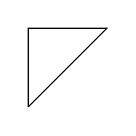
\begin{tikzpicture}
		\draw (0,0) -- (1,1)-- (0,1) -- (0,0);
	\end{tikzpicture}
	\caption[fig:reta]{Primeiro triângulo}
\end{figure}

\begin{figure}[h]
	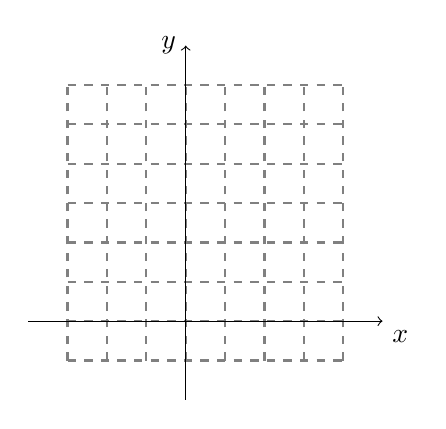
\begin{tikzpicture}[domain=0:4]
		\draw[thick,color=gray,step=.5cm,
		dashed] (-0.5,-.5) grid (3,3);
		\draw[->] (-1,0) -- (3.5,0)
		node[below right] {$x$};
		\draw[->] (1,-1) -- (1,3.5)
		node[left] {$y$};	
	\end{tikzpicture}
	
	\caption[pic:pic2d]{Plano cartesiano}
\end{figure}



\begin{tikzpicture}[domain=0:15]
	\begin{axis}[xlabel=X,ylabel=Y, title=Grafico]% função
		\addplot[samples=200] {1/x}; %Foco na taxa de amostragem
	\end{axis}
\end{tikzpicture}